\section{Background and Motivation}
\label{sec:moti}

\subsection{Agent Serving}

A modern LLM-powered agent follows an \emph{Iterative LLM--Tool Loop}, as shown in Fig.~\ref{fig:workflow}.
In each iteration, the LLM is conditioned on the current context and execution history, and then either emits the final answer or invokes a tool with concrete parameters.
If a tool is invoked, the tool executor runs the invocation, appends the observation back into the session state, and resumes LLM generation on the updated context.

This execution model changes the serving objective.
Unlike isolated LLM requests, agent sessions are long-running, stateful, and highly sequential.
Agent execution is semantically sequential: each step depends on the output of the previous step. In today's agent systems like Codex and Qwen Code, however, this semantic order is typically realized as a physically serialized path: the LLM generates, emits a tool call, waits for the tool result, and then resumes generation.
As a result, LLM generation and tool execution form a single critical path.
Therefore, the agent serving system's latency objective shifts from minimizing token-level latency to minimizing task-level end-to-end (E2E) latency across online sessions, including both average and tail latency.

\subsection{Observation 1: Tool Execution Is Critical-Path}
\label{sec:inefficiencies}

We first measure the latency breakdown of individual agent requests under the most favorable serving condition: one agent request at a time, with no request queueing or resource contention.
We use representative agent workloads from deep research, coding, and AI-for-Science, and run Qwen-DeepResearch-30B on a server with 8 NVIDIA A100-80G GPUs.
As Fig.~\ref{fig:moti:single} shows, LLM generation and tool execution contribute comparable latency in this ideal setting.
Across the evaluated agents, tool execution accounts for 45\%--57\% of agent E2E latency.

\begin{figure}[t]
    \centering
        \centering
        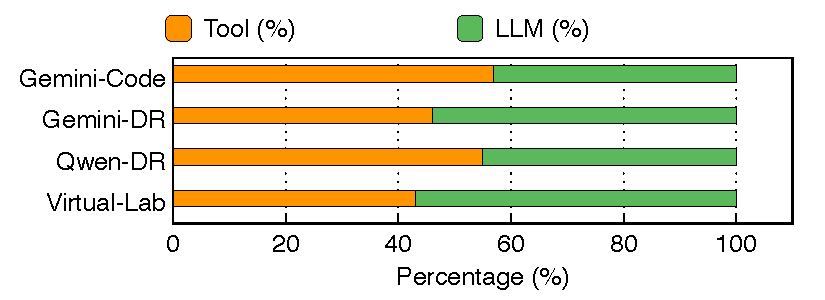
\includegraphics[width=\linewidth]{images/ATC/tool_llm_percentage_solo.pdf}
    \vspace{-0.2in}
    \caption{Breakdown of tool execution and LLM generation.}
    \label{fig:moti:single}
    \vspace{-0.15in}
\end{figure}



This result shows that tool execution is substantial.
Because this semantic order is typically realized as a physically serialized path, the tool portion directly appears on the agent critical path.
Thus, reducing task E2E latency requires reducing the exposed tool time on this serialized path, not only accelerating LLM generation.

\subsection{Observation 2: Future Tool Use Is Predictable}
\label{subsec:opportunities}

Reducing this exposed tool time without changing the agent's semantic order requires knowing concrete future invocations before they appear on the serialized path.
Future tool use is often predictable before the LLM explicitly emits the next tool call.
Agent tool use is generated online by the LLM.
It is not deterministic, but real traces still exhibit structure.
As Fig.~\ref{fig:motifs} shows, real traces show recurring sub-workflow patterns, such as \textit{search} followed by \textit{visit}, \textit{edit} followed by \textit{run test}, \textit{grep} followed by \textit{file\_editor}.
These patterns often carry implicit data dependencies, where subsequent tool call's inputs are already contained in earlier calls' outputs.
For example, 55\% of successful \textit{file\_editor} calls are followed by terminal execution, and in 95\% of web visits the URL is a strict substring of the preceding search output.
This predictability is not limited to tool names.
As Fig.~\ref{fig:moti:arg-source} shows, the measured tool calls are dominated by invocations whose arguments are derived from the prompt or outputs of previous tools rather than generated from scratch by the LLM in the current step.
These derived-argument tool calls are also latency-heavy, making them especially useful targets for reducing exposed tool time.
Therefore, future tool invocations can often be predicted before they appear on the serialized path.

\begin{figure}[t]
    \centering
    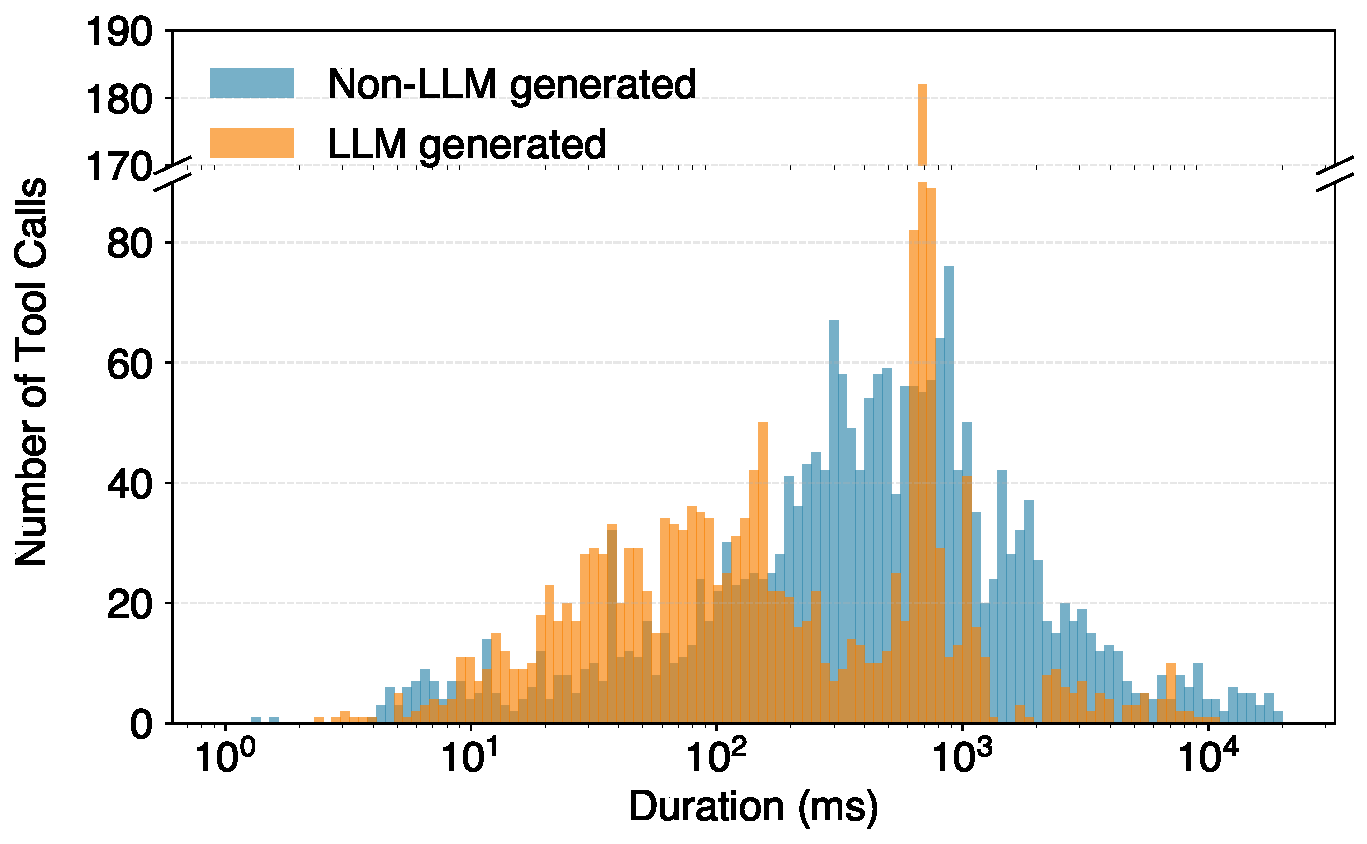
\includegraphics[width=0.98\linewidth]{images/Motivation/histogram_overall.pdf}
    \vspace{-0.1in}
    \caption{Tool execution time histogram. Blue: args from prior outputs; orange: LLM-generated args.}
    \label{fig:moti:arg-source}
    \vspace{-0.1in}
\end{figure}

\subsection{Opportunities and Challenges}
\label{subsec:observation2}

\textbf{Opportunity.} Together, these two observations create an opportunity for serving-level parallelization: the system can reduce substantial exposed tool time by predicting concrete future tool invocations and executing them while the LLM is still generating. Instead of waiting for the LLM to emit every tool call, \sys can execute these invocations speculatively. This speculative execution creates temporal overlap between the tool execution and LLM generation. Through this overlap, the serving system parallelizes tool execution and LLM generation without changing the agent's semantically sequential workflow.
The key is to move concrete tool execution earlier in physical time, not to change the agent's semantic order.
Once a predicted invocation can be instantiated from the observed context, the tool side can start executing it during the LLM generation interval that would otherwise precede the \textbf{authoritative tool call} (i.e., tool calls invoked by LLMs).
If the LLM later emits the same invocation, a completed speculative result can be reused, or an in-flight speculative execution can be promoted, so the session waits only for the remaining tool time instead of the full tool latency.
In this way, predictable control flow and implicit data flow become practical overlap between tool execution and LLM generation.

However, leveraging this opportunity presents two challenges:

\textbf{Challenge 1: Accurate and safe speculative tool execution.} Effective speculation must predict concrete future invocations under uncertainty, not only tool names.
The same pattern can imply different arguments in different sessions, and wrong arguments waste speculative work because the speculative results are not reusable when the authoritative invocation arrives.
A search may be followed by a visit, but the latency benefit only appears if the system chooses the right URL; an edit may be followed by a test, but the command and working directory must match the actual task.
These arguments are often copied or lightly transformed from earlier observations, so the system must recover implicit data-flow from noisy online context.
At the same time, speculative execution must be safe: predicted invocations should not delay, reorder, or otherwise affect authoritative invocations, and speculative actions that violate safety or side-effect constraints should not be admitted for execution.
Thus, the system needs both accurate concrete prediction and policy-compliant speculative execution before predicted tool invocations can be executed safely ahead of authoritative confirmation.

\textbf{Challenge 2: Blind speculation can create LLM--tool phase imbalance.} The second challenge comes from the coupling between the tool phase and the LLM phase: LLM generation runs on shared GPUs and is highly sensitive to workload because its efficiency depends on dynamic resource utilization and memory constraints.
As Fig.~\ref{fig:moti:concurrency} shows, when concurrency grows from one to 192 concurrent sessions, LLM generation time grows by more than 17$\times$, while tool execution time changes only modestly.
Thus, any blind speculation policy that executes predicted tools as soon as possible and admits returning sessions immediately can make many sessions return to the LLM engine earlier and closer together, increasing active LLM load and shifting the bottleneck from the tool phase to the LLM phase.

\begin{figure}[t]
    \centering
    \begin{subfigure}[b]{0.8\linewidth}
        \centering
        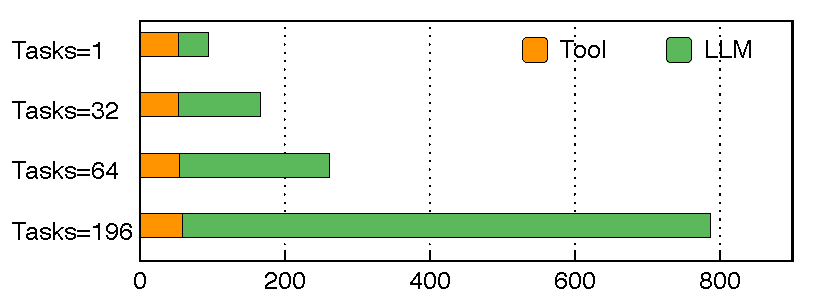
\includegraphics[width=\linewidth]{images/ATC/tool_llm_concurrency_e2elatency.pdf}
        \caption{Absolute E2E time (s)}
        \label{fig:moti:conc-e2e}
    \end{subfigure}
    \begin{subfigure}[b]{0.8\linewidth}
        \centering
        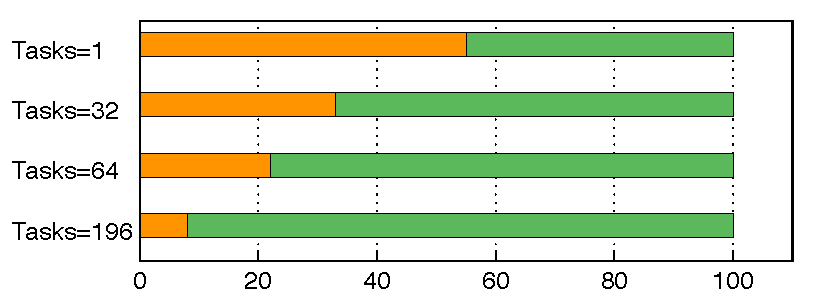
\includegraphics[width=\linewidth]{images/ATC/tool_llm_concurrency_percentage.pdf}
        \caption{Time proportion (\%)}
        \label{fig:moti:conc-percent}
    \end{subfigure}
    \vspace{-0.1in}
    \caption{LLM generation and tool execution have different load sensitivity under concurrent agent tasks.}
    \label{fig:moti:concurrency}
    \vspace{-0.2in}
\end{figure}

This LLM-side sensitivity matters because the balance between the tool phase and the LLM phase is bursty rather than steady during real agent execution.
Each session alternates between tool execution and LLM generation, and these alternations are not aligned across sessions.
As Fig.~\ref{fig:timeline} illustrates, the resulting per-step decode batch size and GPU load fluctuate substantially, so the LLM engine repeatedly moves between under-utilization and overload.

\begin{figure}[t]
    \centering
    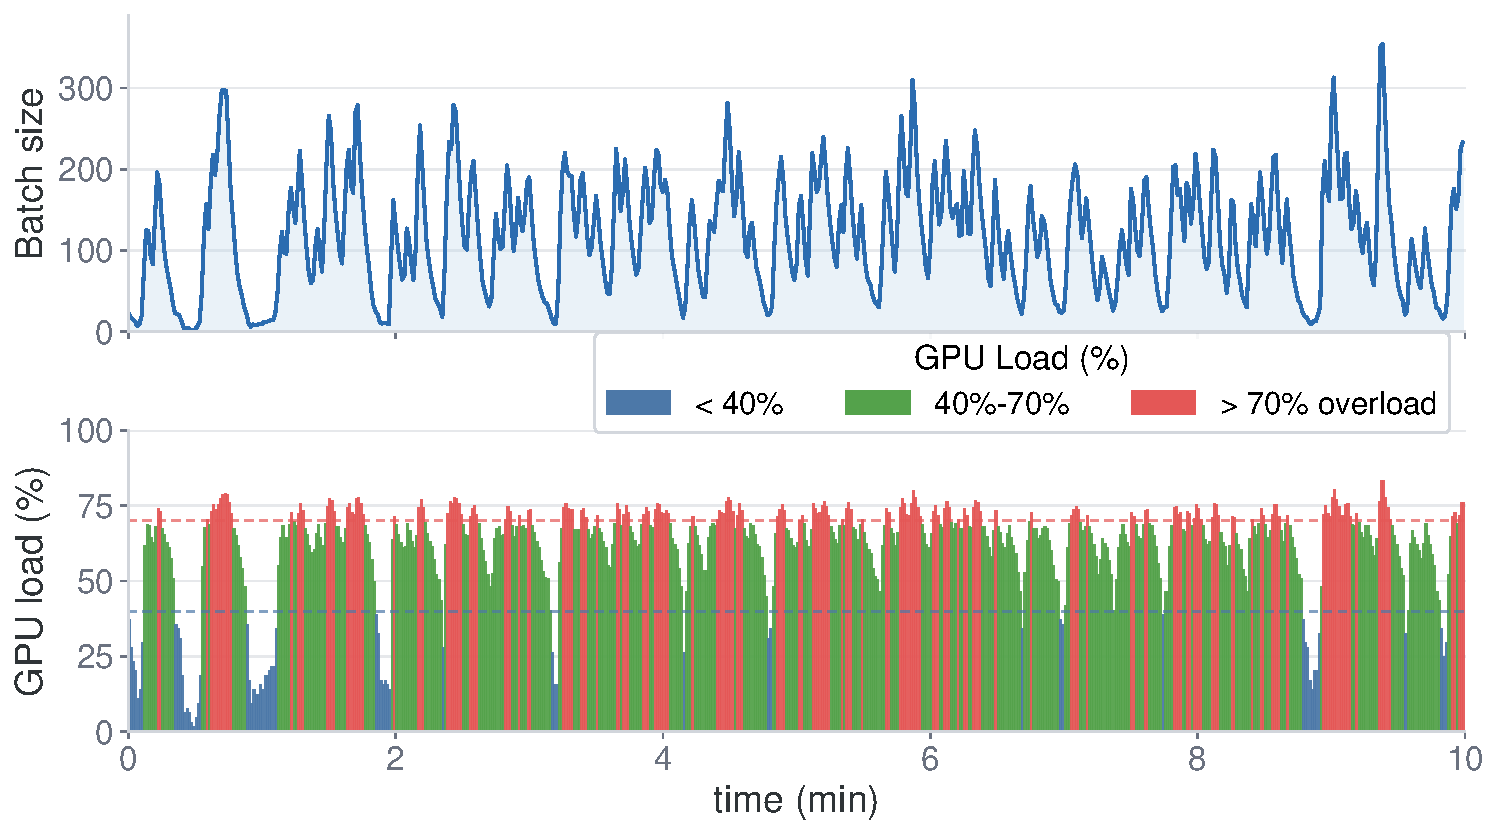
\includegraphics[width=\linewidth]{images/ATC/workload_trace_10min.pdf}
    \vspace{-0.2in}
    \caption{Bursty GPU pressure from alternating LLM generation and tool execution.}
    \label{fig:timeline}
    \vspace{-0.2in}
\end{figure}

Uncoordinated parallelization therefore does not always reduce task-level latency: correct speculation shortens exposed tool time, but blind speculation can make many sessions become ready for LLM generation earlier and closer together, increasing active batch size and creating phase imbalance.
We confirm this effect with a controlled experiment that accelerates tool execution by 2$\times$ while leaving the LLM-side scheduler unchanged; under high load, the extra returning workload slows LLM generation enough to absorb the tool-side gain, and in the worst case makes end-to-end latency worse than the baseline.
Therefore, the system must jointly decide when to execute speculative tool calls and how to pace sessions that return from tool-side into the LLM batch, avoiding phase imbalance that converts tool acceleration into LLM slowdown.

\subsection{Why Existing Systems Are Insufficient}

Existing LLM-serving and agentic-serving systems are tool-unaware and therefore do not address this joint problem.

Agent-level schedulers and general LLM serving engines optimize admission, batching, decoding, or session scheduling~\cite{kwon2023efficient, agrawal2024sarathiserve, duan2024muxserve, qiao2024conserve}.
However, they still treat ready LLM requests as the main scheduling unit and tool execution as an opaque blocking interval.
They do not know which sessions are waiting in tools, when tools will return, whether the tool side is congested, or the context lengths and KV footprints of returning sessions.
Therefore, they cannot smooth active LLM load or pace sessions before they re-enter the LLM engine.

KV cache swap and KV cache management systems optimize memory pressure~\cite{pan2025kvflow, kim2025kvzip, cai2025rkv, yang2025kvlink, prabhu2024vattention}, which is useful when GPU memory capacity limits admission.
However, our timeline experiment shows another common regime for agent serving: SM utilization and compute pressure are high, while GPU memory utilization is not full.
In this regime, KV cache management alone cannot substantially reduce LLM latency growth, because the bottleneck is not simply memory capacity: long-horizon agent tasks spend most of their latency outside the prefill stage.
Thus, LLM-side systems need tool-side state to control future LLM load.

% \subsection{Design Implications}

% These observations lead to two design requirements.
% First, the system should use recurring control-flow patterns and implicit data-flow dependencies to speculatively execute likely future tool invocations, reducing exposed tool latency on the critical path.
% The Pattern Analyzer abstracts dynamic agent behavior into stable invocation sequences and implicit parameter derivation rules.
% The Pattern Tuple abstraction separates the context, prediction, function, and probability fields.
% This decouples control flow from data flow, allowing speculative invocations to run before the LLM emits the authoritative invocation.

% Second, speculation must be coupled with LLM-side scheduling.
% The Online Scheduler should jointly manage authoritative invocations, speculative invocations, and returning LLM generations using both tool-side and LLM-side state.
% This state includes predicted tool completion time, tool congestion, active LLM requests, context length, and KV footprint.
% By deciding when to run speculative work, when to prioritize authoritative tool work, and how to pace sessions returning to the LLM engine, the scheduler can reduce exposed tool time while keeping active LLM load away from under-utilization and overload.
% This joint management is necessary for local tool-side gains to translate into lower task-level end-to-end latency.
